\documentclass{beamer}
\usetheme{metropolis}
\usepackage{graphicx}
\defbeamertemplate*{title page}{customized}[1][]
{
  \usebeamercolor[fg]{titlegraphic}\inserttitlegraphic
  \begin{center}
    \usebeamerfont{title}\inserttitle\par
    \usebeamerfont{subtitle}\usebeamercolor[fg]{subtitle}\insertsubtitle\par
    \bigskip
    \usebeamerfont{author}\insertauthor\par
    \usebeamerfont{institute}\insertinstitute\par
    \usebeamerfont{date}\insertdate\par
  \end{center}
}

\title{Unrolling Recurrent Neural Networks}
\author{Petru Rebeja}
\titlegraphic{
  \begin{center}
    
\includegraphics[width=0.4\textwidth]{../img/iasi-ai-logo.png}
  \end{center}
}
\date{November 14, 2018}
% \logo{
\includegraphics[height=1.5cm]{../img/iasi-ai-logo.png}}
\begin{document}
\maketitle
\begin{frame}
  \frametitle{The shortcomings of a traditional Neural Network \cite{rnn-efectiveness}}
  \begin{columns}
    \begin{column}{0.3\textwidth}
      \begin{center}
        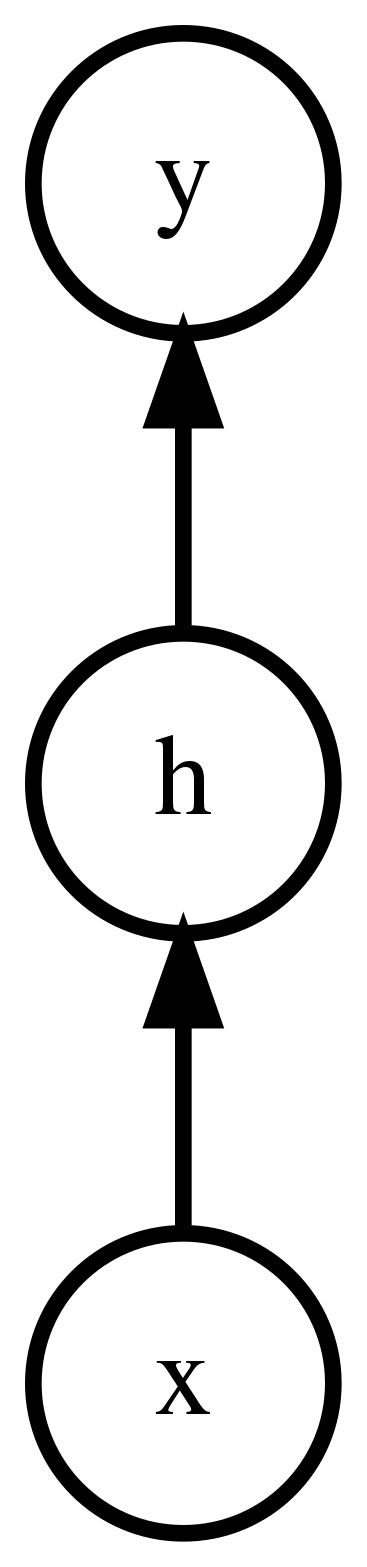
\includegraphics[height=0.6\textheight]{../img/traditional-nn.png}
      \end{center}
    \end{column}
    \begin{column}{0.7\textwidth}
      We all have seen the marvelous success achieved by neural networks (especially Convolutional Networks).
      \pause \\
      However, regardless of their success these networks have some shortcomings which deem them unfit for a wide range of tasks:
      \begin{itemize}
        \item Constrained to a \textbf{fixed size input} and produce \textbf{fixed size output}.
        \item The number of \textbf{computational steps} is \textbf{fixed}.
      \end{itemize}
    \end{column}
  \end{columns}
\end{frame}
\begin{frame}
  \frametitle{Working with data of variable size}
  \begin{itemize}
    \item There are domains (Natural Language Processing for example) where the data samples don't have a fixed size; e.g. \textit{documents} are a \textit{sequence of tokens}. \pause
    \item Furthermore, some tasks require finding temporal patterns/dependencies or patterns/dependencies distributed across some projection of time. \pause
    \item Detecting such patterns/dependencies in a computationally feasible way requires parameter sharing -- a feature which Convolutional Networks are lacking.
  \end{itemize}
\end{frame}
\begin{frame}
  \frametitle{Parameter sharing}
  \begin{itemize}
    \item Allows generalization over samples of different lengths.
    \item Avoids overfitting the sample size from the training set.
    \item Reduces the number of parameters that the model has to learn.
  \end{itemize}
\end{frame}
\begin{frame}
  \frametitle{Using convolutions on sequential data \cite{goodfellow-et-al-2016}}
  \begin{itemize}
    \item Time-delay networks use convolutions across a temporal sequence by applying the same kernel at each time step.
    \item Although this approach allows for parameter sharing across time, \textit{it is shallow}.
    \item The operation only captures a small number of neighboring members of the input.
  \end{itemize}
\end{frame}
\begin{frame}
  \frametitle{Recurrent Neural Networks}
  \begin{itemize}
    \item Are specialized for processing a sequence of values \cite{goodfellow-et-al-2016}
    \item Offer a more powerful way of processing the data \cite{rnn-lecture} and are Turing-Complete \cite{siegelmann1995}
    \item Can process sequences of variable length \cite{goodfellow-et-al-2016}
    \item Are a special case of \textbf{Recursive Neural Networks} which, in turn, are a separate topic (maybe for another presentation).
  \end{itemize}
\end{frame}
\begin{frame}
  \frametitle{Computational Graph for Recurrent Networks}
  \begin{columns}
    \begin{column}{0.3\textwidth}
      \begin{center}
        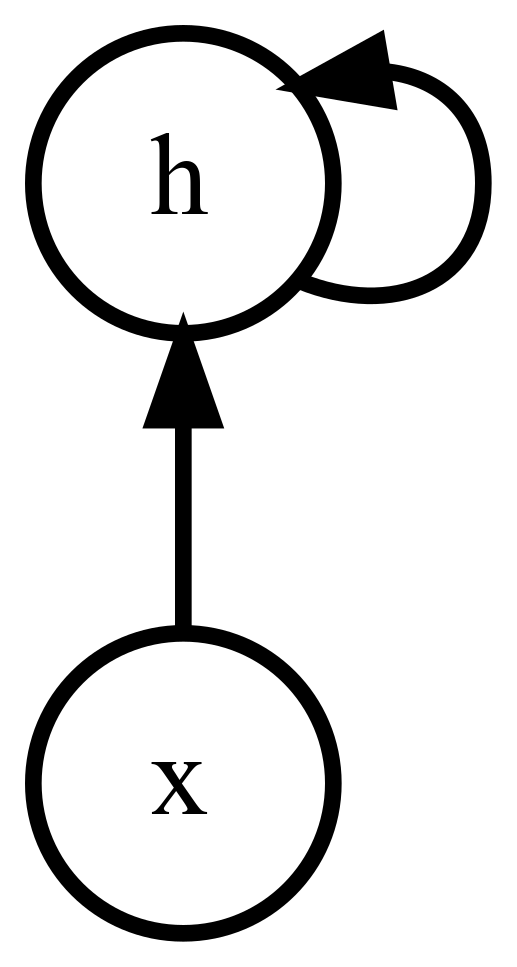
\includegraphics[height=0.6\textheight]{../img/rnn-comp-graph.png}
      \end{center}
    \end{column}
    \begin{column}{0.7\textwidth}
      The theoretical computational graph of a Recurrent Network consists of two parts:
      \begin{enumerate}
        \item The \textit{input} node which receives the current element of the sequence \(x^{(t)}\)
        \item The \textit{hidden} node which gets activated by both \(x^{(t)}\) and hidden node state from previous step \(h^{(t-1)}\)
      \end{enumerate}
    \end{column}
  \end{columns}
\end{frame}
\begin{frame}
  \frametitle{Computational Graph for Recurrent Networks}
  \begin{columns}
    \begin{column}{0.3\textwidth}
      \begin{center}
        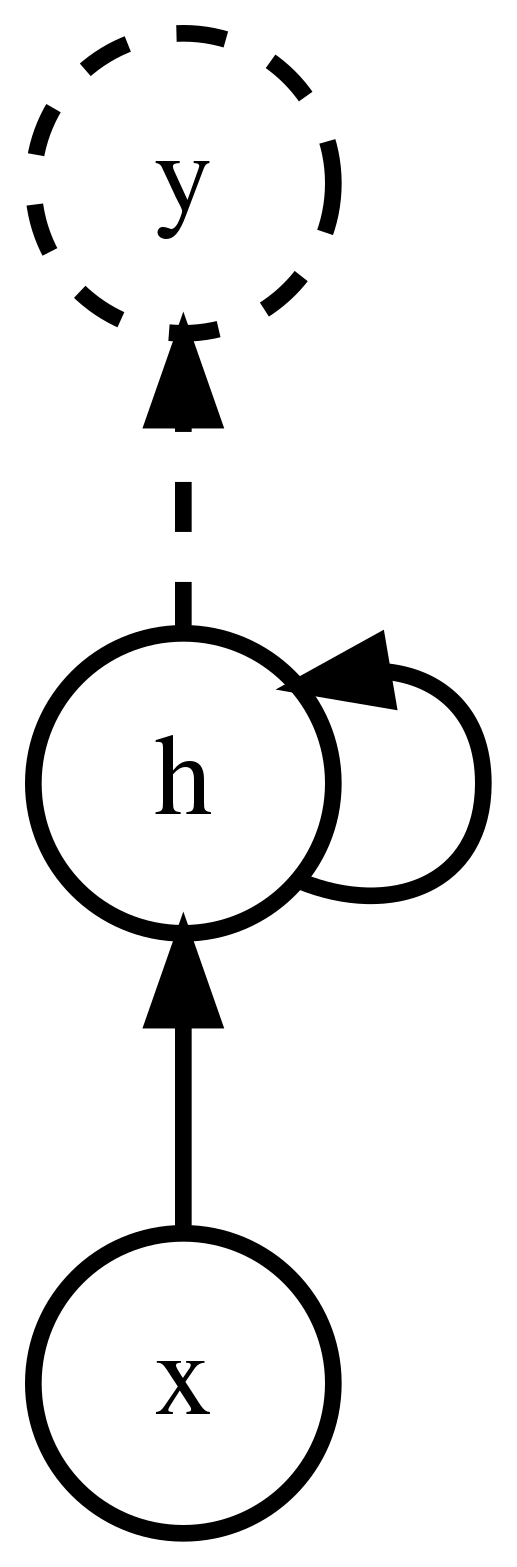
\includegraphics[height=0.6\textheight]{../img/recurrent-nn.png}
      \end{center}
    \end{column}
    \begin{column}{0.7\textwidth}
      In practice we're also interested in outputting some values from the network (e.g. the probability of \(w\) being the next word in the generated sequence) thus we add extra nodes which compute:
      \begin{itemize}
        \item The output for the current element in the sequence
        \item The \textit{loss} value of the output when in training etc.
      \end{itemize}
    \end{column}
  \end{columns}
\end{frame}
\begin{frame}
  \frametitle{Unrolling computational graph}
  \begin{columns}
    \begin{column}{0.3\textwidth}
      \begin{center}
        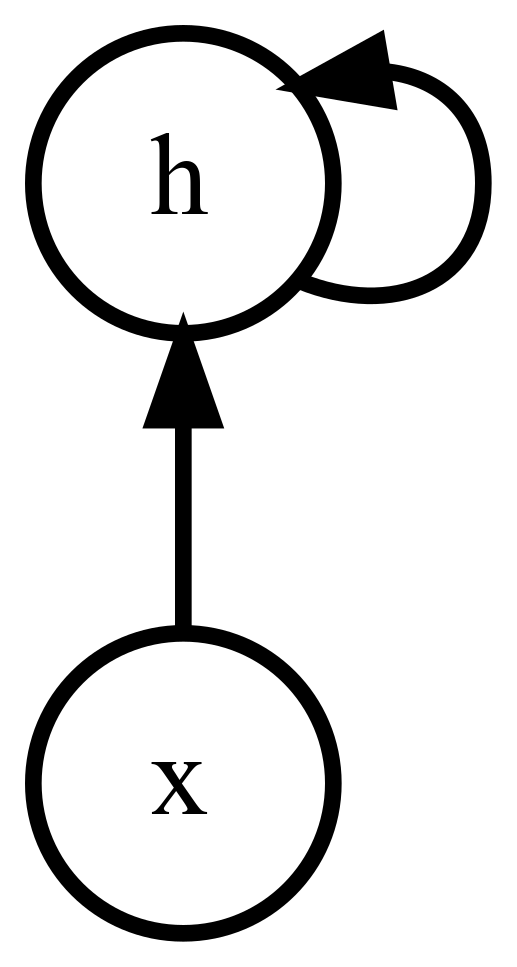
\includegraphics[height=0.6\textheight]{../img/rnn-comp-graph.png}
      \end{center}
    \end{column}
    \begin{column}{0.7\textwidth}
      \begin{enumerate}
        \item The problem with recurrent expressions is that they introduce cycles in the computational graph.
        \item In order to avoid this, the computational graphs of Recurrent Networks are transformed through a process called \textbf{unrolling} or \textbf{unfolding}.
      \end{enumerate}
    \end{column}
  \end{columns}
\end{frame}
\begin{frame}
  \frametitle{Unrolling computational graph}
  This transformation implies copying over a number of times the input, hidden and output nodes and connecting the hidden nodes between them.
  \begin{center}
    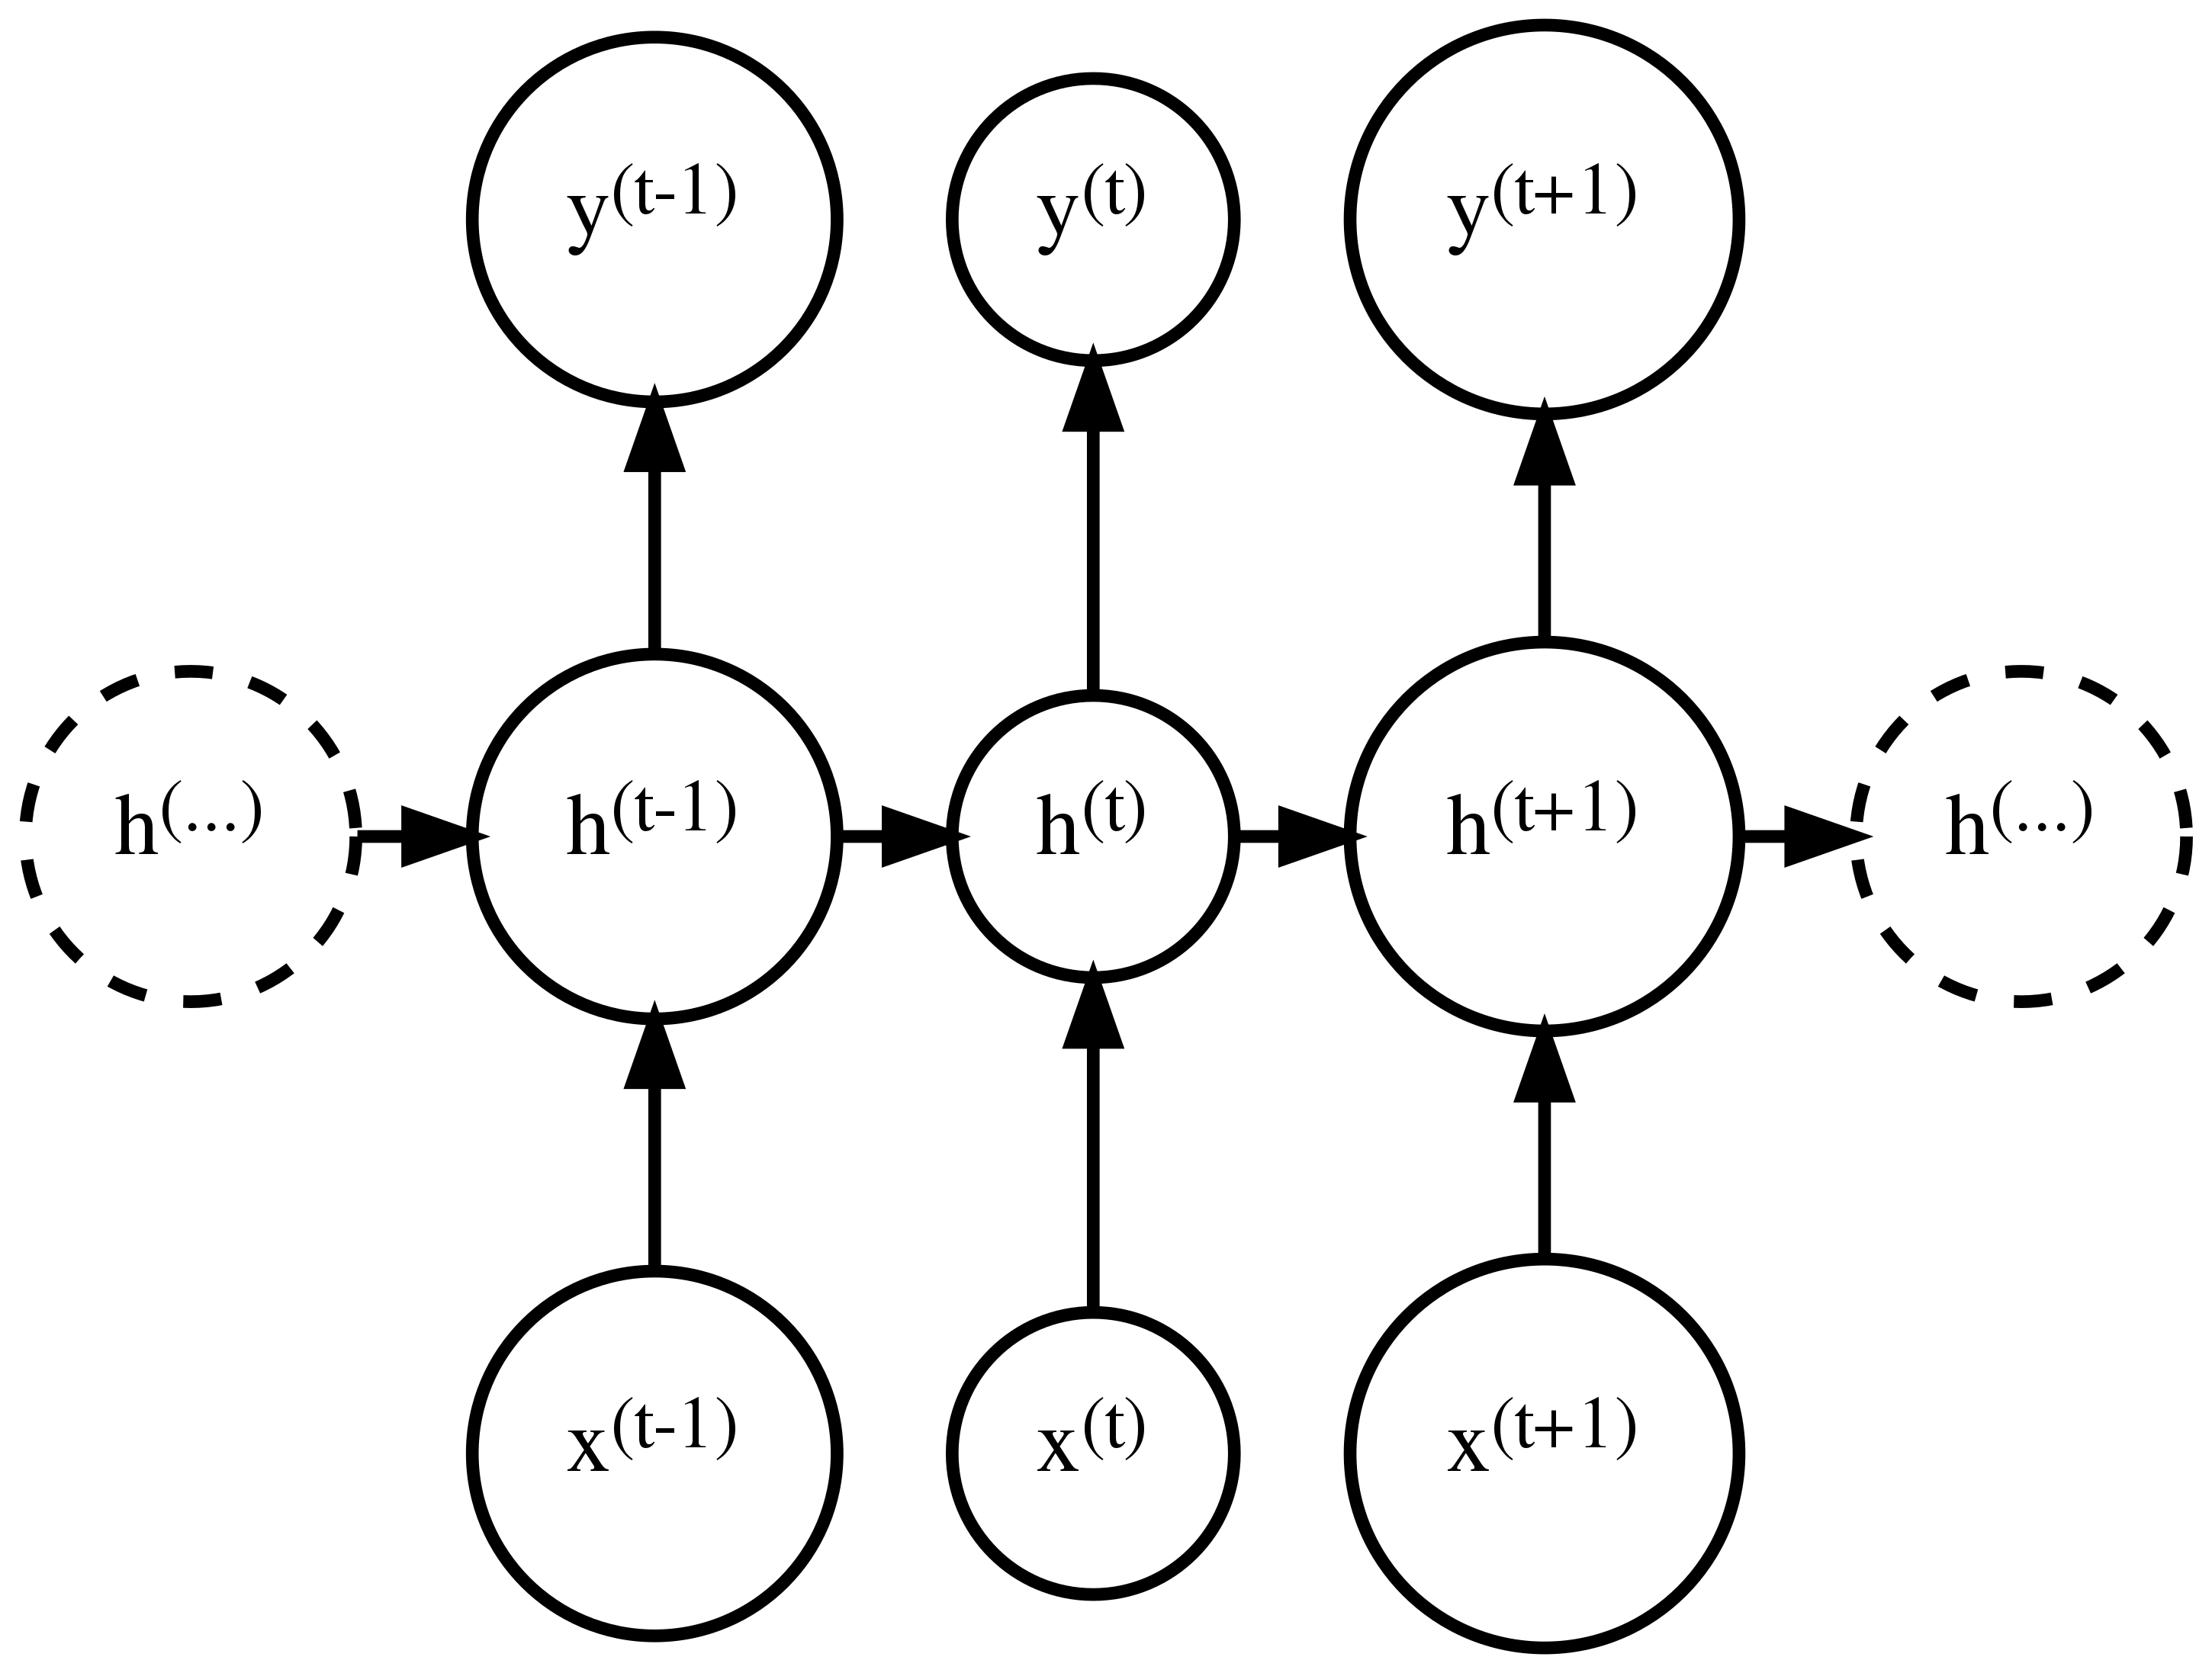
\includegraphics[height=0.6\textheight]{../img/rnn-unrolled.png}
  \end{center}
\end{frame}
\begin{frame}
  \frametitle{Unrolling computational graph}
  The unrolling process introduces two major advantages \cite{goodfellow-et-al-2016}:
  \begin{enumerate}
    \item The input is interpreted as transitions from one fixed size state to another thus the sequence length does not influence neither the model nor the parameter size
    \item \textit{Same} transition function with same parameters can be applied at each step in the sequence
  \end{enumerate}
  Also, unrolling introduces out-of-the box mini-batching.
\end{frame}
\begin{frame}[allowframebreaks]
  \frametitle{Flavors of Recurrent Networks \cite{rnn-efectiveness}}
  \begin{columns}
    \begin{column}{0.3\textwidth}
      \begin{center}
        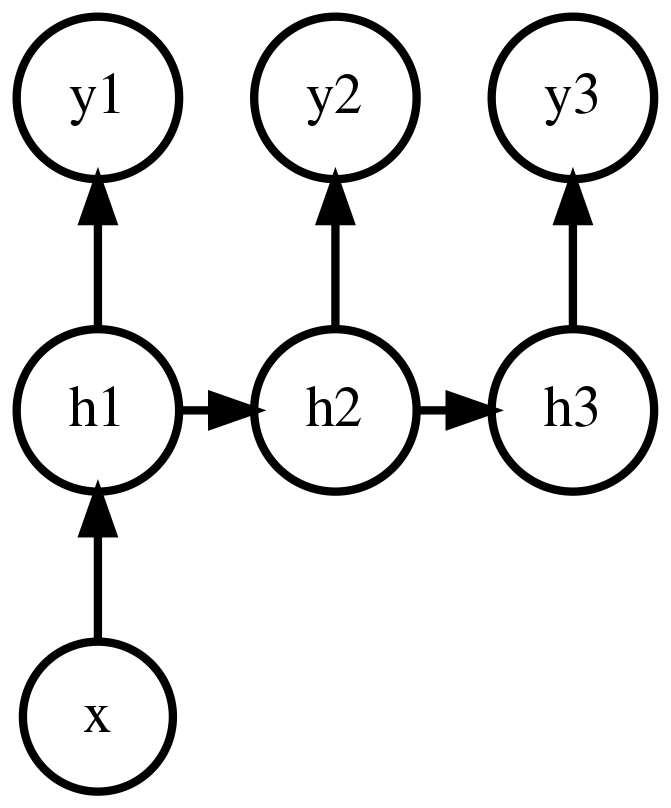
\includegraphics[height=0.5\textheight]{../img/one-to-many.png}
      \end{center}
    \end{column}
    \begin{column}{0.7\textwidth}
      \begin{center}
        \textbf{One to many}
      \end{center}
      \begin{itemize}
        \item Given a fixed size input, the network outputs a sequence of values.
        \item e.g. \textit{Image captioning} - The network takes an image and outputs a sequence of words.
      \end{itemize}
    \end{column}
  \end{columns}
  \framebreak
  \begin{columns}
    \begin{column}{0.3\textwidth}
      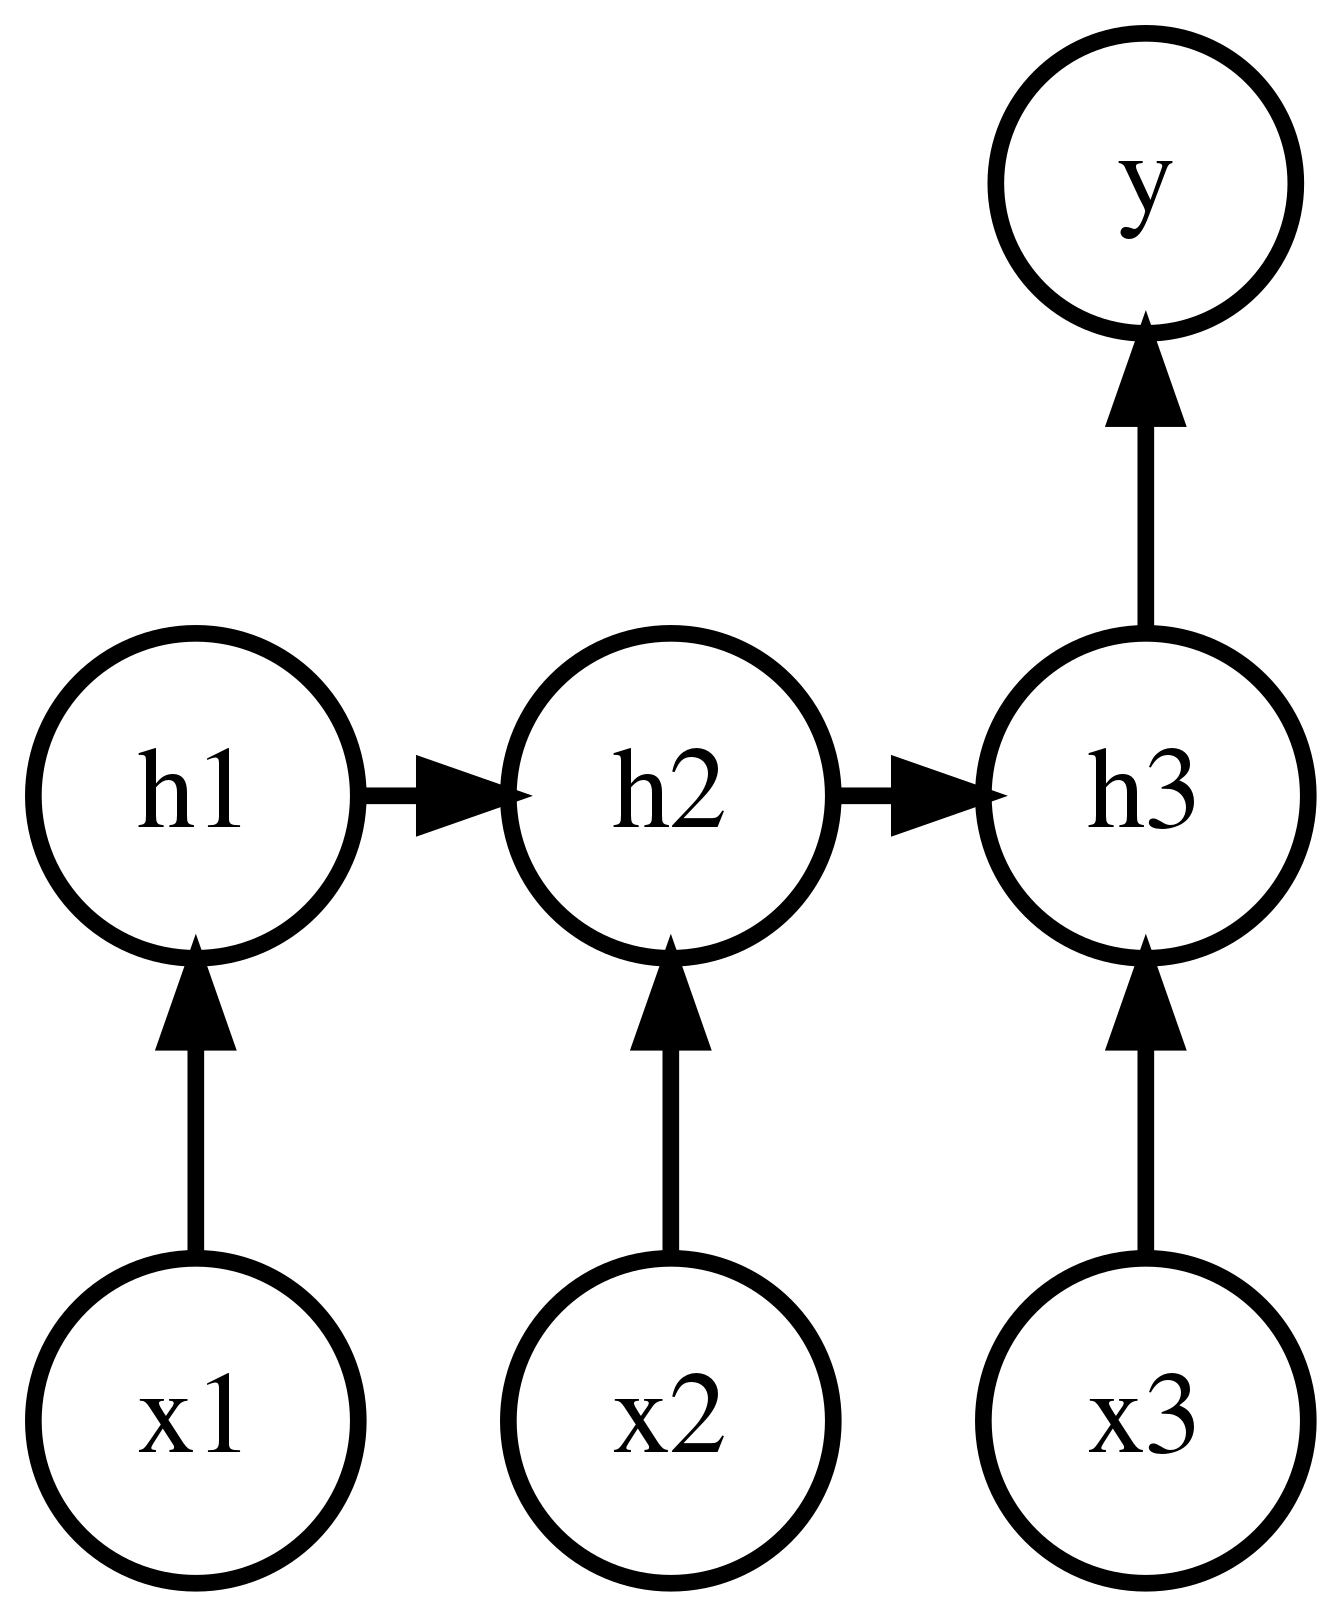
\includegraphics[height=0.5\textheight]{../img/many-to-one.png}
    \end{column}
    \begin{column}{0.7\textwidth}
      \begin{center}
        \textbf{Many to one}
      \end{center}
      \begin{itemize}
        \item Given a sequence of values, the network outputs a fixed size result.
        \item e.g. \textit{Sentiment analysis} - The network takes a sentence (sequence of words) and classifies it as expressing positive, negative or neutral sentiment.
      \end{itemize}
    \end{column}
  \end{columns}
  \framebreak
  \begin{columns}
    \begin{column}{0.4\textwidth}
      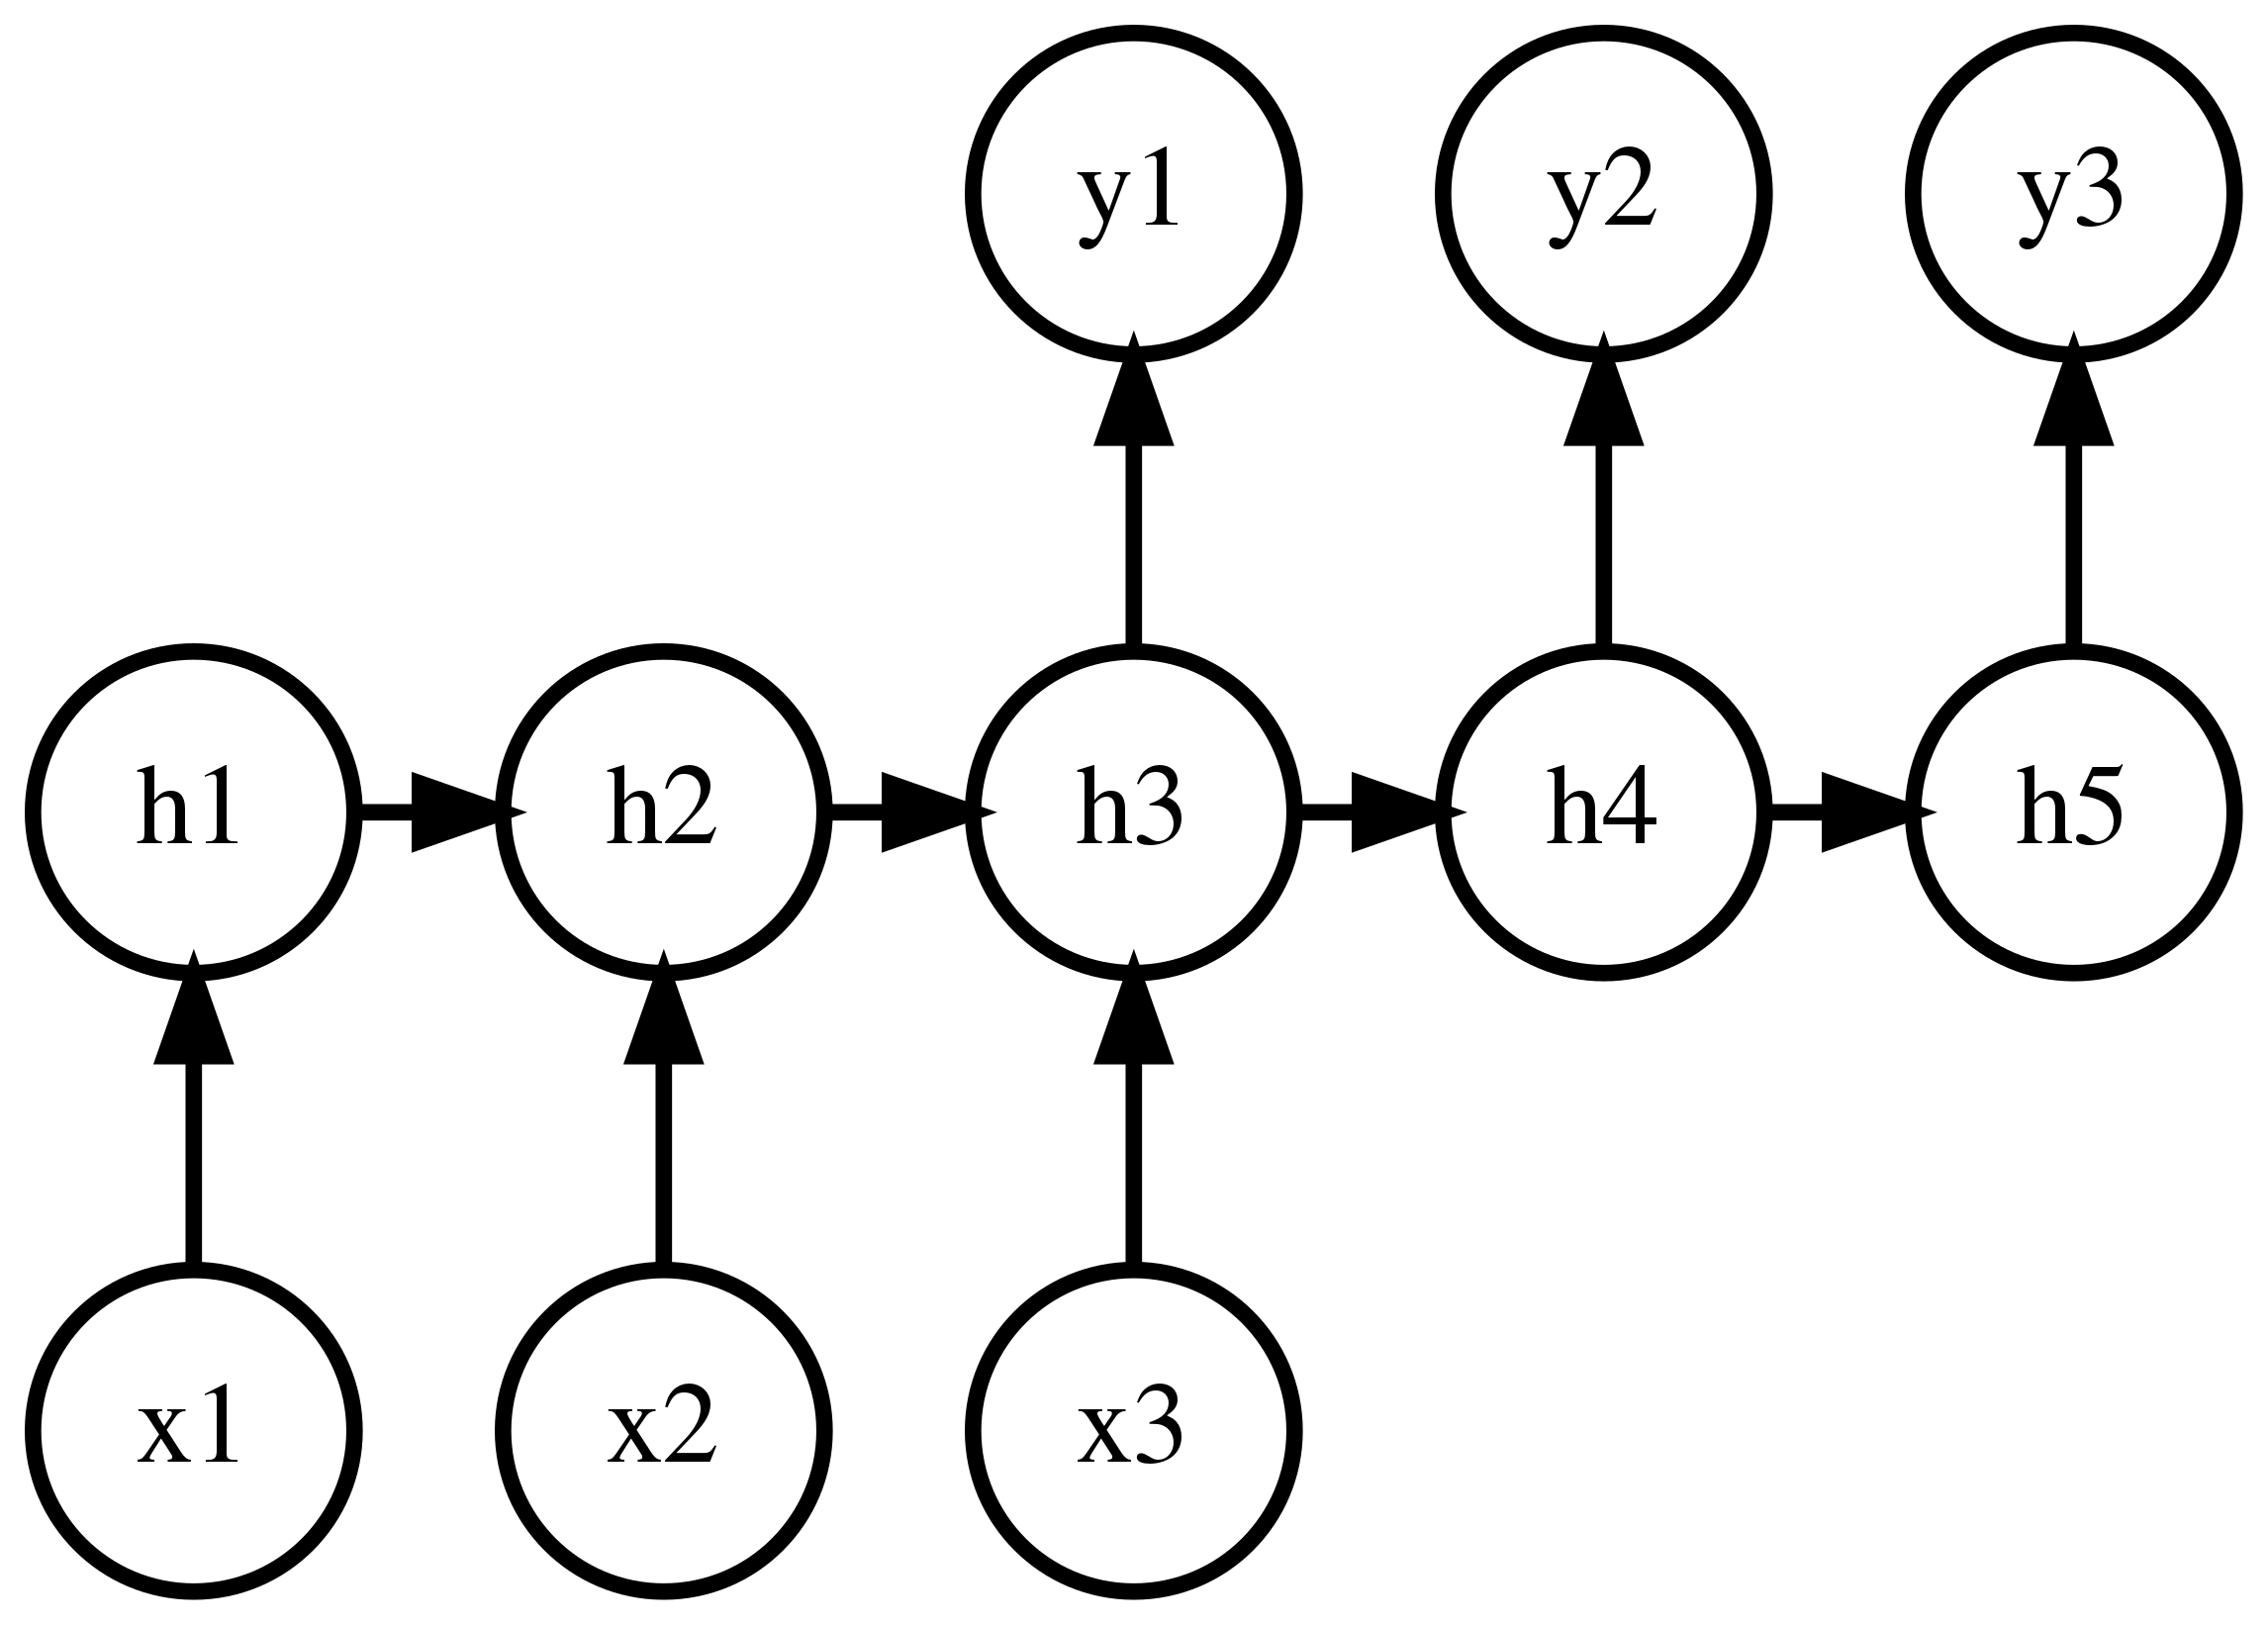
\includegraphics[height=0.4\textheight]{../img/many-to-many-1.png}
    \end{column}
    \begin{column}{0.6\textwidth}
      \begin{center}
        \textbf{Many to many (I)}
      \end{center}
      \begin{itemize}
        \item Given a sequence of values, the network outputs another sequence of values.
        \item e.g. \textit{Machine translation} - The network takes a sentence in English and then outputs a sentence in Romanian.
      \end{itemize}
    \end{column}
  \end{columns}
  \framebreak
  \begin{columns}
    \begin{column}{0.3\textwidth}
      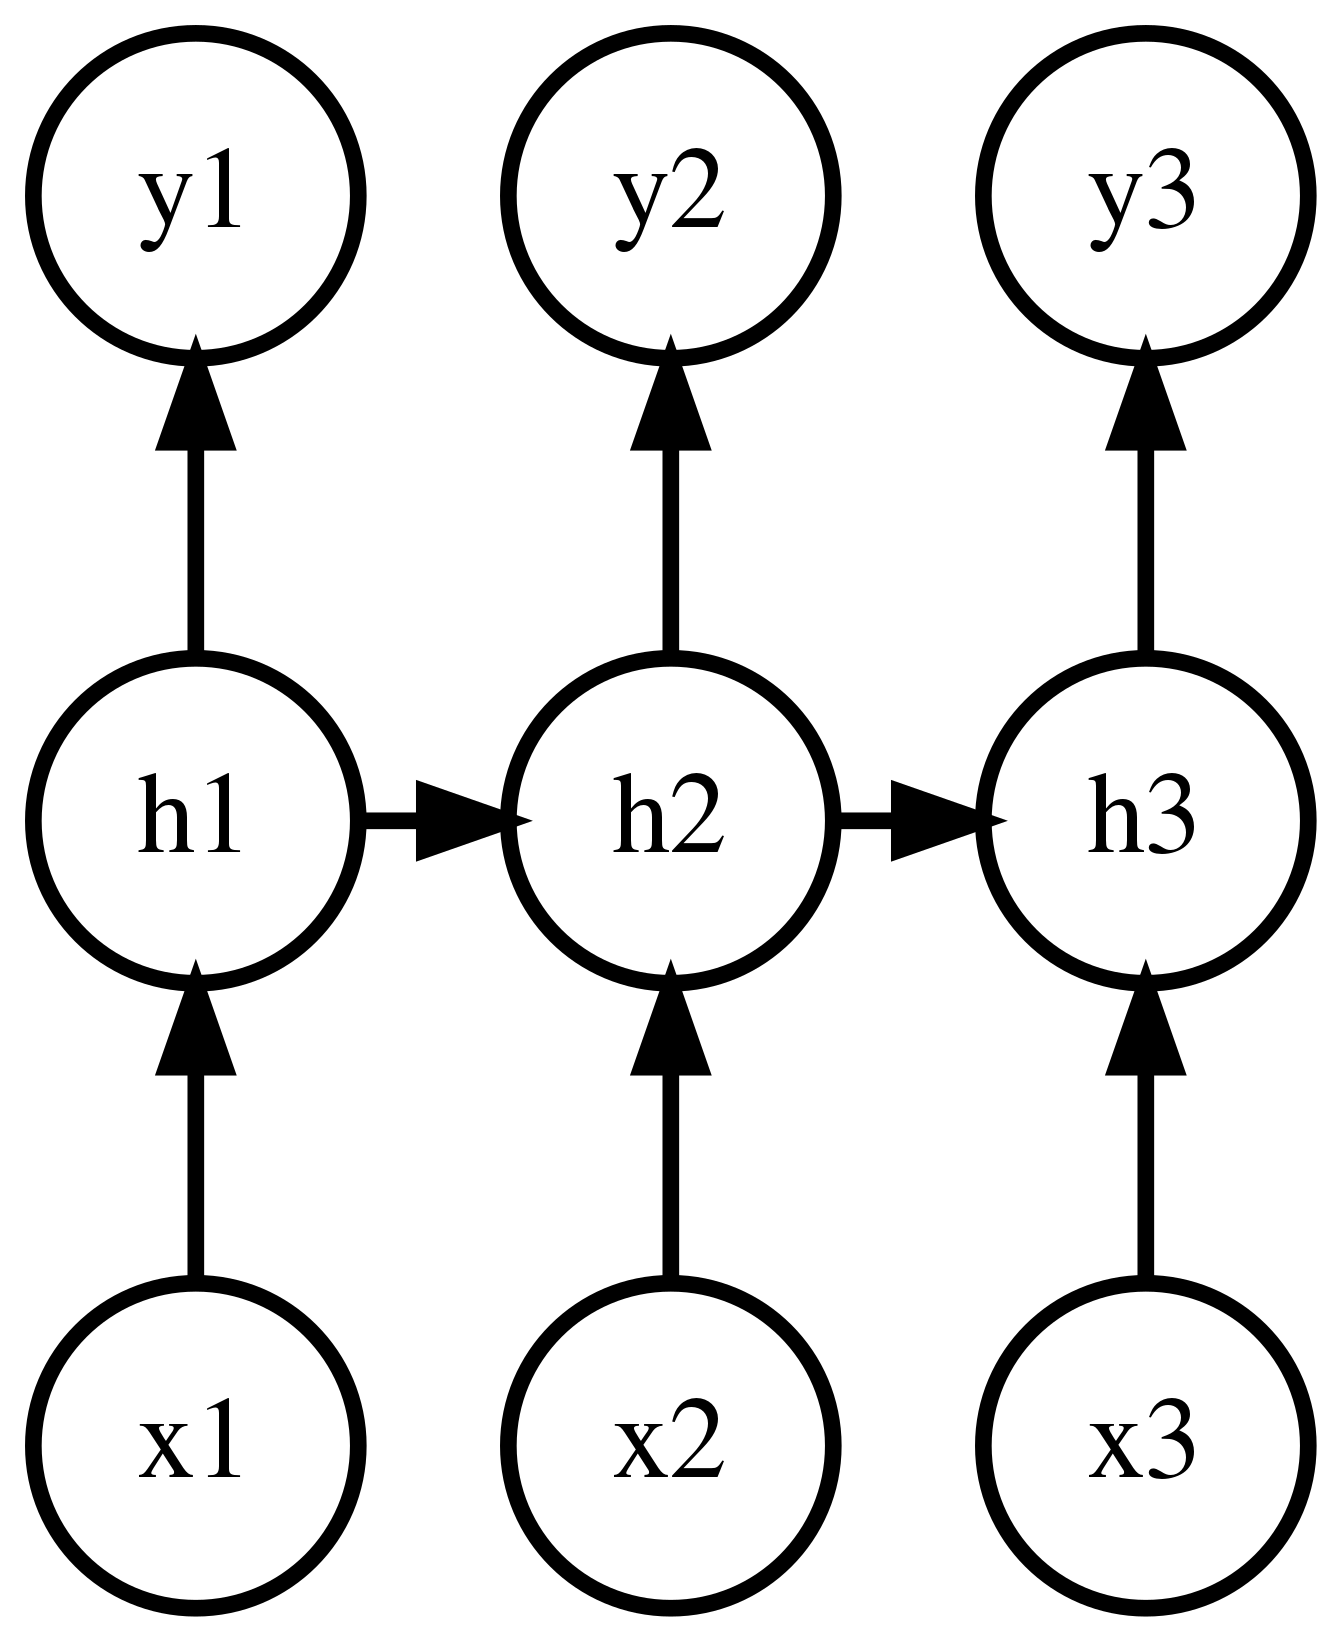
\includegraphics[height=0.5\textheight]{../img/many-to-many-2.png}
    \end{column}
    \begin{column}{0.7\textwidth}
      \begin{center}
        \textbf{Many to many (II)}
      \end{center}
      \begin{itemize}
        \item Given a sequence of values, the network outputs another sequence of values.
        \item e.g. \textit{Video classification on frame level} - The network takes a sequence of video frames and classifies each one based on frame contents \textit{and} the frames before.
      \end{itemize}
    \end{column}
  \end{columns}
\end{frame}
\begin{frame}[allowframebreaks]
  \frametitle{An example}
  Character-level language model with \(tanh\) activation and \(softmax\) normalization \cite{rnn-gist} \cite{goodfellow-et-al-2016}.
  \begin{itemize}
    \item \textbf{Forward pass}
      \begin{enumerate}
        \item Start with some initial state \(h_0\); usually initialized to zeroes
        \item For each \(x^{(t)}\) in the mini-batch calculate:
          \begin{itemize}
            \item Values for the hidden layer
            \item (Normalized) Output probabilities
            \item Loss
          \end{itemize}
        \end{enumerate}
    \framebreak
  \item \textbf{Backward pass} -- Start from the end of the sequence and back-propagate into each node
    \begin{enumerate}
      \item Back-propagate into \(y\)
      \item Back-propagate into \(h\)
      \item Back-propagate through \(tanh\)
      \end{enumerate}
  \framebreak
  \item \textbf{Gradient clipping}
    \begin{itemize}
      \item The recurrence formula is basically an exponentiation of \(W_{xh}\) matrix
      \item Thus when its elements are small they risk \textit{vanishing} and when they are large they may \textit{explode}
      \item A common practice to avoid this is to apply \textbf{clipping}
    \end{itemize}
  \framebreak
  \item \textbf{Parameter update}
    \begin{itemize}
      \item Update model parameters according to the optimization technique
      \end{itemize}
  \end{itemize}
\end{frame}
\begin{frame}
  \frametitle{Thank you!}
\end{frame}
\begin{frame}[allowframebreaks]
  \frametitle{References}
  \bibliographystyle{amsalpha}
  \bibliography{unrolling-rnns}
\end{frame}
\end{document}
%%% Local Variables:
%%% mode: latex
%%% TeX-master: t
%%% End:
